\documentclass{article}
\usepackage[utf8]{inputenc}

\usepackage{mathrsfs}
\usepackage{amsfonts}
\usepackage{amsmath}
\usepackage{amssymb}
\usepackage{graphicx}

\graphicspath{ {./images/} }

\title{Percolation on a $\mathbb{Z}^d$ graph}
\author{Antoine Colonna d'Istria}
\date{March 2021}

\begin{document}

\maketitle

\section{Introduction}

What is percolation? Percolation can be described as the study of graphs which should verify certain properties (we say they are "regular"), where we remove some vertex with a certain probability. It is a very useful theory as it simulates a lot of different situations in physics: electromagnetism (etc)...

More precisely, we will be interested by the study of the connected set of such a graph, what we call "clusters" and how it behaves in relation of the probability p chosen. There will be what we call a critical probability that divides the problem in three cases.

We will be only concerned by bond percolation, that is to say by the removal of the edges and not the vertexes.

\subsection{Definition of percolation}
Let G = (V,E) be a graph with a certain "regularity" (it 'looks' the same from any vertex). We call percolation the process of removing a number of edges with a probability $\textit{p}\in [0,1]$ to get a random subgraph G'=(V,E')

An edge of G is called open if it is not in G', and closed if it is. 

We consider the following space : $(\Omega, \mathscr{F}, P_p)$ where :
\begin{gather*}
(i) \ \Omega = \prod_{e \in \mathbb{E}}{\{0,1\}} \\
(ii) \ \mathscr{F}=\\
(iii) \ P_p = \prod_{e \in \mathbb{E}}{\mu_{e}}
\end{gather*}

where, $\mu_{e}$ is a Bernoulli measure with a parameter $p\in [0,1]$ for each $e\in\mathbb{E}$. In fact we name configurations the space associated, subset of $\Omega$ where :

$$
\omega(e) = \left\{
    \begin{array}{ll}
        0 & \mbox{if e is closed}\\
        1 & \mbox{if e is open}
    \end{array}
\right.
$$

We call $K(\omega)$ the subgraph of open edges.

\begin{figure}
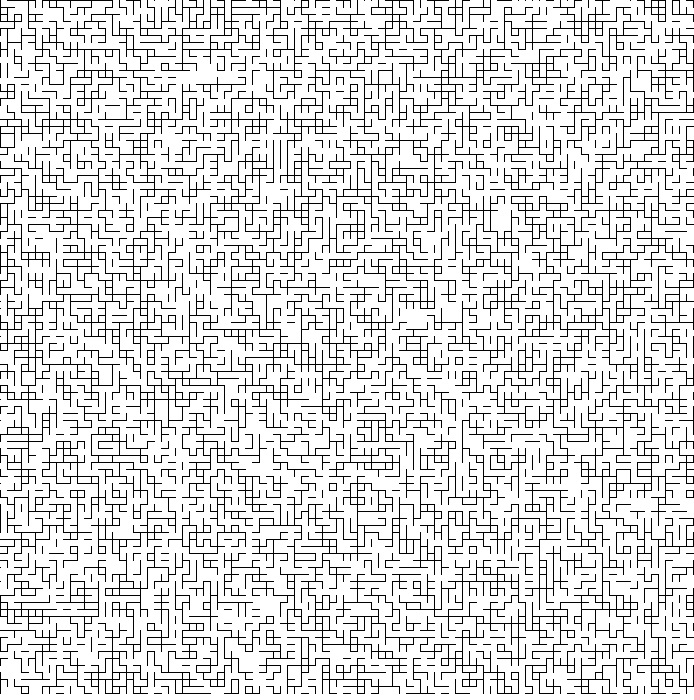
\includegraphics[scale=0.75]{percolation0}
\centering

\caption{Example of a percolation of a $\mathbb{Z}^2$ graph (100x100), where p = 0.5}
\end{figure}


\subsection{Another point of view}
We had seen the point of view where we choose p and then we percolate. But we can see the other way and define some random uniform variables for each edge between $0$ and $1$, and then discriminate depending on $p$

Let $(X(e), e\in\mathbb{E})$ a family of uniform random variables in $[0,1]$. For $p \in [0,1]$, we say :

$$
\eta_p(e) = \left\{
    \begin{array}{ll}
        0 & \mbox{if $X(e) < p$ (closed)}\\
        1 & \mbox{otherwise (open)}
    \end{array}
\right.
$$

Thus, we can see how it is going. As p is going through $0$ to $1$, the edges are removed going from a complete graph G to a total isolate graph with no edges $(V, \varnothing)$

IMAGES

\subsection{Studying open clusters}
\subsubsection{Definition}
We call an open cluster a connected component of the subgraph of open clusters and we write $C(x)$ the open cluster connected to a vertex $x \in V$. They form a partition of $K(w)$.

Now, we take $\mathbb{L}^d=(V,E)$ and $V=\mathbb{Z}^d$. Points are connected when at a Manhattan distance of $1$.
As the graph is regular (invariant by translation), the distribution of edges doesn't depend on any particular vertex, so we can fix a point, the origin for instance, and only study $C=C(0)$

\subsubsection{The Critical phenomenon}
Let study the connected clusters of $\mathbb{L^d}$ depending on $p$. Is there an infinite cluster?
As we saw, we can only restrain ourself to the origin. Is $C = C(0)$ an infinite cluster?
What we will see is that it exists a critical value $p_c\in [0,1]$ such as: \\

(i) \ if $p < p_c$, then $C$ is almost always an infinite cluster (subcritical phase) \\
(ii) \ if $p > p_c$, then $C$ is almost always not an infinite cluster (supercritical phase) \\
(iii) \ if $p = p_c$, then we are in the critical phase, the most interesting case \\

We can write this as: \\
$$\theta(p) = P_p(|C|=\infty)$$
$$
\theta(p) = \left\{
    \begin{array}{ll}
        0 & \mbox{if $p < p_c$}\\
        1 & \mbox{if $p > p_c$}
    \end{array}
\right.
$$
Where the critical probability p is equal to:
$$p_c = sup\{p \ | \ \theta(p)=0\}$$

\subsubsection{Trivial case of d = 1}

Let's study $\mathbb{L}^1$. We know for sure that if $p < 1$, then almost certainly there will be a closed edge to left of the origin, and to the right. Thus, there will always never an infinite cluster if $p < 1$. If $p = 1$, there will be always an infinite cluster.

\subsubsection{Case of $d \geq 2$}

To prove we have a critical phenomenon, we could restrain ourself to $d = 2$.

PROOF

Let's study $\mathbb{L}^d$ for $d \geq 2$.
We have:
$$\Phi(p)=P_p(|C|=\infty)$$
the probability that there exists an infinite cluster. We have :
$$
\Phi(p) = \left\{
    \begin{array}{ll}
        0 & \mbox{if $\theta(p)=0$}\\
        1 & \mbox{if $p > p_c$}
    \end{array}
\right.
$$
It can be translated as the fact that there is almost certainly an infinite cluster if the probability that there is an infinite cluster at the origin is not zero, and is almost impossible otherwise. It shows how studying at a certain vertex (here the origin) is equivalent to study for any vertex (which can be far more difficult). It is proven by using the zero-one law which states that if an event, here "the graph contains an infinite cluster" is not dependant upon the states of any finite collection of edges. So, the probability $\Phi(p)$ is equal to $0$ or $1$.

We have two cases ;
If $\theta(p)=0$, the distribution of probability being the same everywhere, $\Phi(p)$ should be equal to $0$.
If it is not zero, then it means $\Phi(p)$ is greater than zero, and it is then $1$.

So the critical phenomenon being proved for the origin, we deduce that there is a probability $p_c$, where under this probability, there is almost never an infinite cluster, if below there is almost always an infinite cluster.

\subsection{Some useful inequalities}

Definition: Increasing Event

We say that $\Psi(p)$ is an increasing function of p if :
In a measurable pair, $(\Omega, \mathscr{F})$, for $w, w' \in \mathscr{F}$
$$w \leq w' \implies \Psi(w) \leq \Psi(w')$$
for a certain order $\leq$ when $w \implies w'$

And $\Psi(p)$ is decreasing if $-N$ is increasing \\

First inequalities :
If $N$ is an increasing random variable on $(\Omega, \mathscr{F})$, then : \\
If $p_1 \leq p_2$ and $\mathbb{E}_{p_1}(N) < \infty$ and $\mathbb{E}_{p_2}(N) < \infty$ then $\mathbb{E}_{p_1}(N) \leq \mathbb{E}_{p_2}(N)$ \\

If $A$ is an increasing event in $\mathscr{F}$ then
(ii) If $p_1 \leq p_2$ then $P_{p_1}(N) \leq P_{p_2}(N)$ \\

Second inequalities, FKG inequalities :

If $X$ and $Y$ are increasing (decreasing) random variables and $\mathbb{E}_p{(X^2)} < \infty$ and $\mathbb{E}_p{(Y^2)} < \infty$, then \\
(iii)
$$\mathbb{E}_p(XY) \geq \mathbb{E}_p(X)\mathbb{E}_p(Y)$$

If $A$ and $B$ are increasing (decreasing) events, then \\
(iv)
$$\mathbb{P}_p(A \cap B) \geq \mathbb{P}_p(A)\mathbb{P}_p(B)$$

If  $X$ is increasing and $Y$ is decreasing random variables and $\mathbb{E}_p{(X^2)} < \infty$ and $\mathbb{E}_p{(Y^2)} < \infty$, then \\
(v)
$$\mathbb{E}_p(XY) \leq \mathbb{E}_p(X)\mathbb{E}_p(Y)$$

If $A$ is increasing and $B$ is decreasing (or the other way) events, then \\
(vi)
$$\mathbb{P}_p(A \cap B) \leq \mathbb{P}_p(A)\mathbb{P}_p(B)$$



\end{document}
